\documentclass[border=12pt]{standalone}
\usepackage{tikz}
\usetikzlibrary{shapes.geometric, arrows.meta, positioning, calc, fit, backgrounds}
\usepackage{fontspec}
\setmainfont{DejaVu Sans}

\begin{document}
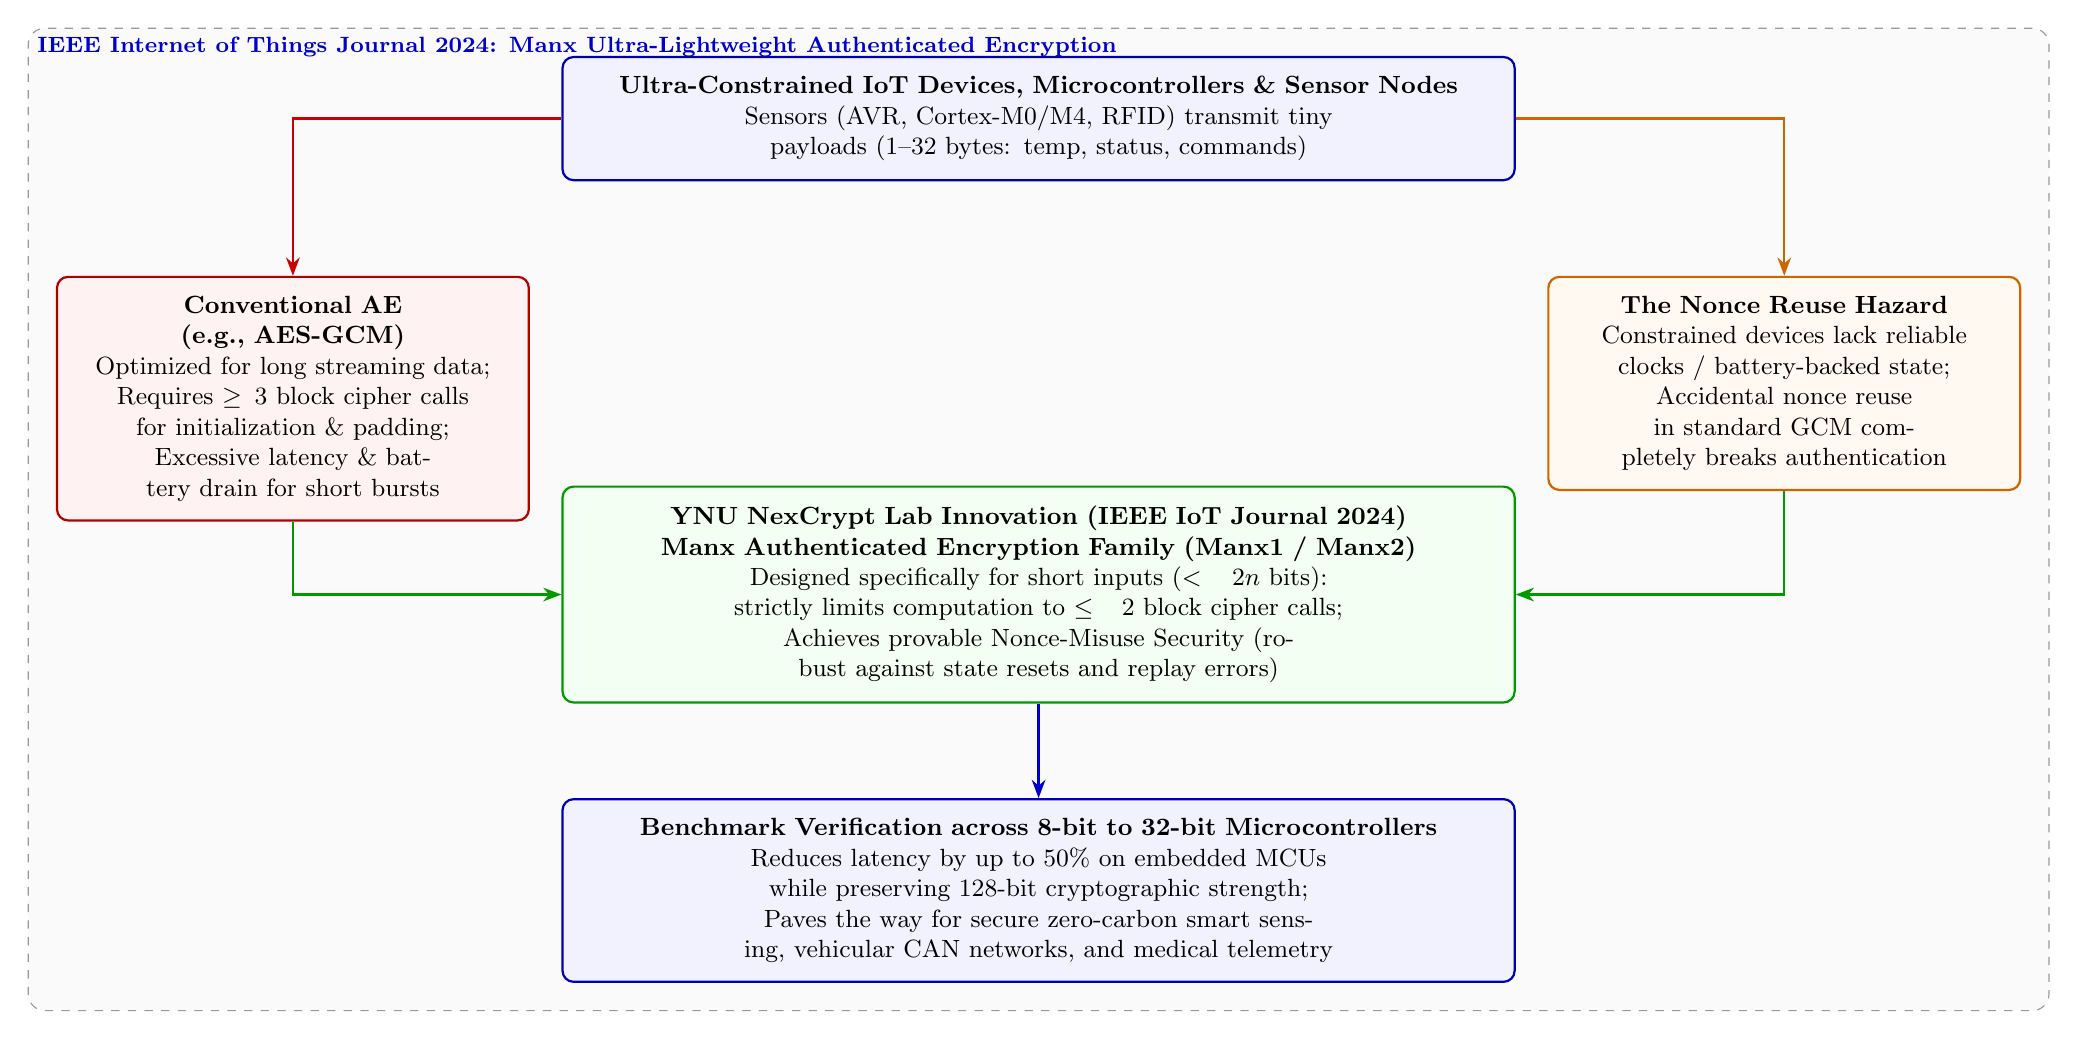
\begin{tikzpicture}[
    font=\small,
    >=Stealth,
    node distance=1.2cm,
    block/.style={rectangle, draw=blue!70!black, fill=blue!5, rounded corners=4pt, thick, align=center, inner sep=7pt},
    alertblock/.style={rectangle, draw=red!70!black, fill=red!5, rounded corners=4pt, thick, align=center, inner sep=7pt},
    greenblock/.style={rectangle, draw=green!60!black, fill=green!5, rounded corners=4pt, thick, align=center, inner sep=7pt},
    amberblock/.style={rectangle, draw=orange!80!black, fill=orange!5, rounded corners=4pt, thick, align=center, inner sep=7pt},
    groupbox/.style={draw=black!40, dashed, rounded corners=6pt, fill=black!2, inner sep=10pt}
]

    % Top: The Ultra-Constrained IoT Challenge
    \node[block, text width=11.6cm] (iot) {\textbf{Ultra-Constrained IoT Devices, Microcontrollers \& Sensor Nodes}\\Sensors (AVR, Cortex-M0/M4, RFID) transmit tiny payloads (1--32 bytes: temp, status, commands)};

    % Left: Standard AE Schemes (AES-GCM / OCB)
    \node[alertblock, below left=1.2cm and 0.4cm of iot, text width=5.5cm] (standard) {\textbf{Conventional AE (e.g., AES-GCM)}\\Optimized for long streaming data;\\Requires $\ge 3$ block cipher calls for initialization \& padding;\\Excessive latency \& battery drain for short bursts};

    % Right: Nonce-Misuse Catastrophe
    \node[amberblock, below right=1.2cm and 0.4cm of iot, text width=5.5cm] (nonce) {\textbf{The Nonce Reuse Hazard}\\Constrained devices lack reliable clocks / battery-backed state;\\Accidental nonce reuse in standard GCM completely breaks authentication};

    \draw[->, thick, red!80!black] (iot) -| (standard);
    \draw[->, thick, orange!80!black] (iot) -| (nonce);

    % Middle: Proposed Manx Mode
    \node[greenblock, below=1.2cm of $(standard)!0.5!(nonce)$, text width=11.6cm] (manx) {\textbf{YNU NexCrypt Lab Innovation (IEEE IoT Journal 2024)}\\\textbf{Manx Authenticated Encryption Family (Manx1 / Manx2)}\\Designed specifically for short inputs ($< 2n$ bits): strictly limits computation to $\le 2$ block cipher calls;\\Achieves provable Nonce-Misuse Security (robust against state resets and replay errors)};

    \draw[->, thick, green!60!black] (standard) |- (manx);
    \draw[->, thick, green!60!black] (nonce) |- (manx);

    % Bottom: Results
    \node[block, below=1.2cm of manx, text width=11.6cm] (results) {\textbf{Benchmark Verification across 8-bit to 32-bit Microcontrollers}\\Reduces latency by up to 50\% on embedded MCUs while preserving 128-bit cryptographic strength;\\Paves the way for secure zero-carbon smart sensing, vehicular CAN networks, and medical telemetry};

    \draw[->, thick, blue!80!black] (manx) -- (results);

    \begin{scope}[on background layer]
        \node[groupbox, fit=(iot) (standard) (nonce) (manx) (results), label={[anchor=north west, font=\footnotesize\bfseries, blue!80!black]north west:IEEE Internet of Things Journal 2024: Manx Ultra-Lightweight Authenticated Encryption}] {};
    \end{scope}

\end{tikzpicture}
\end{document}
